	\documentclass[10pt,oneside]{CBFT_book}
	% Algunos paquetes
	\usepackage{amssymb}
	\usepackage{amsmath}
	\usepackage{graphicx}
	\usepackage{libertine}
	\usepackage[bold-style=TeX]{unicode-math}
	\usepackage{lipsum}

	\usepackage{natbib}
	\setcitestyle{square}

	\usepackage{polyglossia}
	\setdefaultlanguage{spanish}
	



	\usepackage{CBFT.estilo} % Cargo la hoja de estilo

	% Tipografías
	% \setromanfont[Mapping=tex-text]{Linux Libertine O}
	% \setsansfont[Mapping=tex-text]{DejaVu Sans}
	% \setmonofont[Mapping=tex-text]{DejaVu Sans Mono}

	%===================================================================
	%	DOCUMENTO PROPIAMENTE DICHO
	%===================================================================

\begin{document}

% =================================================================================================
\chapter{Gases clásicos ideales}
% =================================================================================================


% =================================================================================================
\section{Fluidos clásicos --reacomodar--}
% =================================================================================================

Empezamos con las funciones de distribución (en el ensamble canónico). Sabemos que
\[
	\left( \frac{\euler^{-\beta V}}{Z_N} \right)d^3q_1 d^3q_2 ... d^3q_N = 
	\text{ \# de microestados tales que '1' está en $\vec{q}_1$, etc. }
\]
donde los momentos están integrados y se cumple 
\[
	V = \sum_{i<j}^N v_{ij}.
\]
Pero ahora 
\begin{multline*}
	\left[ \int d^3q_{l+1} d^3q_{l+1} ... d^3q_{N} \frac{\euler^{-\beta V}}{Z_N} \right] d^3q_1 d^3q_2 ... d^3q_l 
	=\\
	\text{ \# de partículas tales que '1' está en $\vec{q}_1$, la 'l' en $q_l$ y las otras en cualquier parte } 
\end{multline*}

Como las partículas son indistinguibles agregamos 
\[
	\frac{N!}{(N-l)!} \left[ \int d^3q_{l+1} d^3q_{l+1} ... d^3q_{N} \frac{\euler^{-\beta V}}{Z_N} \right] 
	d^3q_1 d^3q_2 ... d^3q_l = \text{ \# de partículas ... } 
\]
y así definimos
\[
	\rho^{[1]}( q_1,...,q_l, V, T ) \equiv \frac{N!}{(N-l)!} \frac{1}{Z_N} \int d^{3N}q_{l+1} ...  d^{3N}q_N 
	\euler^{-\beta V}
\]
que es la función de distribución de $l$ cuerpos.
\[
	\rho^{[1]}( q_1, V, T ) = \frac{N}{Z_N} \int d^{3N}q_2 ...  d^{3N}q_N \euler^{-\beta V}
\]
y entonces
\[
	\int dq_1 \rho^{[1]}( q_1, V, T ) = N \qquad \text{ normalización }
\]
\notamargen{$ \rho^{[1]} = cte.$ entonces $N=\int dq_1 \rho^{[1]} $ y $N/V = \rho^{[1]} $, lo cual es muy razonable.}

Definimos 
\[
	\rho^{[l]} = \left( \frac{N}{V} \right)^l g^{[l]} \qquad g^{[l]} = \frac{\rho^{[l]}}{\rho^l} 
	\qquad N = \frac{N}{V} \int dq_1 g^{[1]}( q_1 )
\]
\notamargen{ $g^{[l]}$ es una especie de densidad relativa. }

\subsection{Análisis de $g^{[2]}(\vec{q}_1,\vec{q}_2)$}

Se puede medir mediante scattering de rayos X.
Con un potencial esférico
\[
	V(\vec{q}_1,\vec{q}_2) = V( |\vec{q}_1-\vec{q}_2| ) = V(q)
\]
donde $q$ es coordenada relativa  y entonces 
\[
	\rho^{[2]} = \left( \frac{N}{V} \right)^2 g^{[2]}( q_1, q_2 ) = 
	\left( \frac{N}{V} \right)^2 g( q )
\]
\[
	\int dq_1 dq_2 \rho^2 g^{[2]} = N(N-1) \qquad \qquad 4\pi \int dq \: q^2 \rho g(q) = N(N-1)
\]
\[
	4\pi \int dq q^2 \rho g(q) \cong N \qquad \text{ esféricas }
\]

Ahora $g(q)\rho^2$ da la probabilidad de que dada una partícula en 'O' tenga otra a distancia $q$. Es una probabilidad
conjunta.
\notamargen{ $\rho^{[2]} = \rho^{[2]}(q_1,q_2,V,T)$ pero en un gas ideal es 
$ \rho^{[1]}(q_1,V,T) \rho^{[1]}(q_2,V,T) $ lo que significa que no hay correlación.}
Los casos límite serán 
\begin{itemize}
	\item $q \to 0 \quad g \to 0 \quad $ Por la repulsión del carozo
	\item $q \to \infty \quad g \to 1  \quad $ Por el desvanecimiento del potencial (a gran distancia el sistema se 
ve 	homogéneo)
\end{itemize}

DIBUJO

Para un líquido da algo como esto. El valor de $ \sigma $ sería como la separación a primeros vecinos.

Para un sólido sería algo como esto (ver debajo), donde los picos están asociados a la separación entre primeros, segundos y
terceros vecinos.

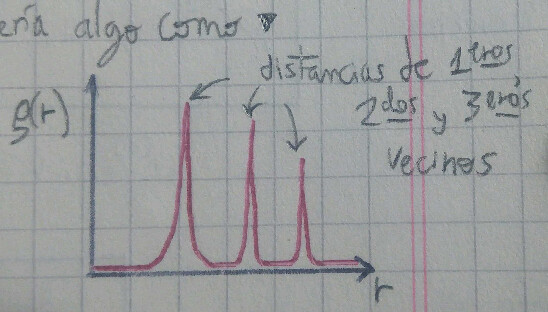
\includegraphics[scale=0.3]{images/1625623567.jpg}

\subsection{La termodinámica y $g(q)$}
\[
	\Ham = K(p) + V(q)
\]
\begin{multline*}
	E = <\Ham> = \frac{ \int d^{3N}p \int d^{3N}q \euler^{-\beta K - \beta V} (K+V) }
	{\int d^{3N}p \int d^{3N}q \euler^{-\beta K - \beta V}} = \\
	\frac{ \int d^{3N}p \int d^{3N}q \euler^{-\beta K - \beta V} K + \int d^{3N}p \int d^{3N}q \euler^{-\beta K - 
	\beta V} V }{ \int d^{3N}p \euler^{-\beta K } \int d^{3N}q \euler^{- \beta V} }
\end{multline*}
\[
	E = <K> + \frac{ \int d^{3N}q \euler^{-\beta V} V }{Z_N}
\]
\[
	-\dpar{}{\beta} \log Z_N = -\frac{1}{Z_N} \int d^{3N}q \euler^{-\beta V} (-V) = kT^2 \dpar{}{T}
\]
\[
	E = <K> + kT^2 \dpar{}{T}(\log Z_N)
\]
\[
	<V> =  \frac{ \int d^{3N}q \euler^{-\beta V} V }{Z_N} = 
	\frac{ \int d^{3N}q \euler^{-\beta \sum_{i<j}^N V_{ij} } \sum_{i<j}^N V_{ij} }{Z_N} =
	\sum_{i<j}^N \frac{ \int d^{3N}q \euler^{-\beta V } V_{ij} }{Z_N}
\]
\notamargen{La sumatoria en $ V_{ij} $ me la puedo sacar de encima.}
\[
	<V> = \frac{(N-1)N}{2} \frac{ \int d^{3N}q \euler^{-\beta V } V_{ij} }{Z_N}
\]
Metemos la expresión para $\rho^{[2]}$
\[
	\rho^{[2]} = \frac{N!}{(N-2)!} \frac{1}{Z_N} \int dq^3_3 ... d^3q_N \euler^{-\beta V}
\]
\[
	<V> = \frac{(N-1)N}{2} \int d^3q_1 d^3q_2 \left( 
	\frac{1}{Z_N} \int dq^3_3 ... d^3q_N \euler^{-\beta V}\right) V_{ij}
\]
\[
	<V> = \frac{(N-1)N}{2} \int d^3q_1 d^3q_2  \frac{(N-2)!}{N!}
	\rho^2 g^{[2]}(q_1,q_2) V_{12}
\]
\[
	<V> = \frac{1}{2} \int d^3q_1 d^3q_2 \rho^2 g^{[2]}(q_1,q_2) V_{12} =
	\frac{1}{2} \int 4 \pi dr r^2 \rho N  g(r) V(r)
\]
\[
	<V> = \frac{N^2}{2V} \int 4 \pi r^2 g(r) V(r) dr
\]
\[
	E = \frac{3}{2} NkT + \frac{N\rho}{2} \int_0^\infty 4 \pi r^2 g(r) V(r) dr
\]
siendo la integral del rhs la energía de interacción de una partícula con las demás sumada sobre todas las partículas.

La determinación de la presión se hace merced a 
\[
	p = -\dpare{A}{V}{N,T}, \quad A = -kT \log [Q_N(V,T)] 
	\qquad p = kT \frac{1}{Q_N} \dpar{}{V}[Q_N(V,T)]
\]
\notamargen{$A=T-TS$ y entonces $dA = dU-TdS-SdT = -pdV + \mu dN -SdT$ y entonces $p=-\partial A/\partial V$}
pero la dependencia del volumen se halla en la parte espacial de modo que 
\[
	p = kT \frac{1}{Z_N} \dpar{}{V}[ Z_N(V,T) ]  
\]
\[
	Z_N = \int d^{3N}q \euler^{\beta V}  = 
	\int_0^{V^{1/3}} \hspace*{-1em} dq_1 \int_0^{V^{1/3}} \hspace*{-1em} dq_2 ... \int_0^{V^{1/3}} 
	\hspace*{-1em} dq_{3N} \euler^{-\beta \sum_{i<j}^N V_{ij}(q_{ij}) }
\]
y cambiando variables con $ r = q/V^{1/3} $ que lleva a $ dq = V^{1/3} dr $
\[
	Z_N = V^N \int_0^1 d^{3N}r \euler^{-\beta \sum_{i<j}^N V_{ij}(V^{1/3}r_{ij}) }
\]


% \bibliographystyle{CBFT-apa-good}	% (uses file "apa-good.bst")
% \bibliography{CBFT.Referencias} % La base de datos bibliográfica

\end{document}
